\documentclass[
12pt, % Main document font size
a4paper, % Paper type, use 'letterpaper' for US Letter paper
headinclude,footinclude % Extra spacing for the header and footer
]{article}

\usepackage[
pdfspacing, % Makes use of pdftex’ letter spacing capabilities via the microtype package
dottedtoc, % Dotted lines leading to the page numbers in the table of contents
nochapters,
]{classicthesis} % The layout is based on the Classic Thesis style

%\usepackage{arsclassica}
\usepackage[german, english]{babel}
\usepackage[T1]{fontenc}
\usepackage[utf8]{inputenc} 
\usepackage{graphicx} 
\graphicspath{{Figures/}} 
\usepackage{enumitem} 
\usepackage{subfig}
\usepackage{amsmath,amssymb,amsthm}
\usepackage{hyperref}
\usepackage{varioref}
\usepackage{geometry}
\usepackage{framed}
\usepackage{tabularx, booktabs}
\usepackage{cprotect}
\usepackage{fancyvrb}
\usepackage{lipsum}
\usepackage{libertine}
\usepackage{titlesec}

\newcolumntype{Y}{>{\centering\arraybackslash}X}

\makeatletter
\newcommand{\verbatimfont}[1]{\renewcommand{\verbatim@font}{\ttfamily#1}}
\makeatother

\hypersetup{
%draft, % Uncomment to remove all links (useful for printing in black and white)
colorlinks=true, breaklinks=true, bookmarks=true,bookmarksnumbered,
urlcolor=webbrown, linkcolor=RoyalBlue, citecolor=webgreen, % Link colors
pdftitle={Enhanced Botero model documentation}, % PDF title
pdfauthor={\textcopyright}, % PDF Author
pdfsubject={}, % PDF Subject
pdfkeywords={}, % PDF Keywords
pdfcreator={pdfLaTeX}, % PDF Creator
pdfproducer={LaTeX with hyperref and ClassicThesis} % PDF producer
}

\newcommand{\modfont}[1]{\begingroup\color{red}#1\endgroup}


\begin{document}
\verbatimfont{\footnotesize}
\pagenumbering{gobble}
\title{\rmfamily\normalfont\spacedallcaps{Enhanced Botero Model Documentation}}
\author{\spacedlowsmallcaps{\href{mailto:mail@dionhaefner.de}{Dion H\"afner}}}
\date{\today}

\maketitle

\tableofcontents
\clearpage
\newcommand{\sectionbreak}{\clearpage}
\pagenumbering{arabic}
\pagestyle{plain}
\section{First Steps}
\subsection{Installation}
To start, just clone the \href{https://github.com/dionhaefner/cces-sem-botero}{git repository} containing this project to your local hard drive.

You will need to have Python 2.7 or 3.x installed, along with the usual scientific packages like NumPy, Matplotlib and Pandas. Additionally, parts of the project are written in Cython, so you will need to have this library installed as well. A convenient way to get all this is Anaconda Python, which is available for all major OS, and free of charge for non-commercial use. Another highly recommended package that is not included with Anaconda Python is Seaborn, which provides high-end data visualization. You can get this either from source or run

\begin{verbatim}
    $ pip install seaborn
\end{verbatim}

\noindent from your favorite Unix-style command line. Without Seaborn, all graphical output will be much less pretty, and violin plots are replaced by simple box plots.

If you cannot or do not want to install Anaconda Python, but have Python >= 2.7 and the package manager pip installed, you may run (with \verb|sudo| as needed)

\begin{verbatim}
    $ pip install -r requirements
\end{verbatim}

\noindent in the main folder of this project. This should automatically install all the necessary requirements.

After you have installed the prerequisites, you will probably have to compile the Cython parts of the module once. To do this, execute

\begin{verbatim}
	$ python setup.py build_ext --inplace
\end{verbatim}

\noindent If none of the commands threw any errors you are ready to start simulating!
\subsection{Usage}

The goal with this package was to create a software that is both easy to use and easy to modify. The simplest work flow for running simulations with this code would be:

\begin{enumerate}
	\item Customize the model parameters in the file \verb|constants.py|, as defined in the array \verb|_PARAMETERS| (or just keep the default values).
	\item Call \verb|python main_constant.py| (simulation with constant population size), and grab a cup of coffee.
	\item The output will be found in a new folder \verb|output| and will contain the mean genes of the populations and their standard deviation in every time step, and a detailed plot every few time steps (may be specified in the \verb|constants.py|).
\end{enumerate}

\noindent For runs with variable population size, you also need to specify two \verb|.csv|--files, containing the mean genes of the starting population and their standard deviation (output of a run with constant population size). You have to pass the name of these files via the command line:

\begin{verbatim}
    $ python main_variable.py <mean-file>.csv <std-file>.csv
\end{verbatim}

\noindent Output is then being printed to the folder \verb|output_var|.

You will probably want to run many different simulations while varying some parameters, and keeping the rest constant. To automate this task, it is more convenient to pass parameters from command line (e.g.\ via a shell script) than to change them in the \verb|constants.py| file. Luckily, \emph{every} parameter that can be specified in the \verb|_PARAMETERS| array can be overwritten from command line, e.g. by calling

\begin{verbatim}
    $ python main_constant.py --population_size 10000 --mu 0.0001
\end{verbatim}

\noindent You can receive a full list of options by calling

\begin{verbatim}
    $ python main_constant.py --help
\end{verbatim}

\subsection{Making changes to the code}

Most of the code of the project is just regular Python code, which should be pretty easy to modify. However, there currently is also one file written in Cython (a module that allows to mix C and Python code), \verb|animal.pyx|, for performance reasons. To have any of the changes to this file take effect you will have to compile it again by running

\begin{verbatim}
    $ python setup.py build_ext --inplace
\end{verbatim}

\noindent The following table gives a short overview on the purpose of each source file:

\vspace{20pt}
\begin{tabularx}{\textwidth}{l | X}
	File & Description \\ \midrule
	constants.py & Sets model constants and parameters for other modules to import, and parses the command line. Change the default values here. \\
	main\_constant.py & Main wrapper to be called for a run with constant population size. \\
	main\_variable.py & Main wrapper to be called for a run with variable population size. Has two additional required command line parameters (mean and standard deviation of the start genes).\\
	setup.py & Compiles the cythonized parts of the project. Needs to be called to have changes to .pyx files take effect.\\
	example.py & Demonstrates the usage of the project's classes. \\
	src/iterate\_population.py & Called by the main wrapper. Operates on given Population and Environment instances. Main time step controller. \\
	src/output\_population.py & Handles file output and plotting. \\
	src/environment.py & Implements Environment class. \\
	src/animal.pyx & Implements Animal class (cythonized). \\
	src/population.py & Implements Population class.
\end{tabularx}

\section{Model Description}
This section is supposed to give a quick introduction to the model as proposed by Botero et al, and the modifications of the model that were done in this code (\modfont{typeset in red}, full list of modifications in \ref{sec:mod}). For a much more complete and detailed consideration refer to their original paper, \cite{botero}.

\subsection{General purpose}
The Botero model simulates a population of a species and their genetic adaptation to their environment. A population consisting of $N$ animals (usually about 5,000), each with their own set of genes, is generated and put into a periodic environment with certain parameters like frequency $R$, predictability $P$, amplitude $A$, and random noise $B$ (for the additional parameter $O$ see \ref{sec:mod}). Of special interest is the predictability $P$ of the environment: The animals can always measure the current state of the environment, $E$, and a \emph{cue} $C$, telling them how a future state may develop (which does not need to be true for $P<1$ -- or may even be anti-correlated for $1 \leq P < 0$). Each animal may develop a certain \emph{strategy} concerning how to adapt their phenotype to the environmental cue, if at all.

Newly born animals inherit their parents' genes, with a chance of random mutation. In a first step, the total number of animals in the population is held constant -- if too many children are born, some of them randomly die, and if too few are born, random entities are cloned. This has the purpose to quickly find the 'best' gene composition without risking the populations extinction with every evolutionary misstep. To make sure that the best genetic composition is eventually adapted throughout the population, the number of offspring of each animal is based on how well the animal has been adapted to its environment throughout its lifetime.

As soon as a set of \emph{good} genes is found, it can be used as a starting condition for runs with a variable population size. In these runs, the environment the animals are put into may change. This is the main thing that Botero et al.~examined: By which amount may the environment change in order to allow the population to continue its existence?

\modfont{This modified version also features \emph{multiple} environments, and allows for migration between them. This way, it can be examined whether migration may be a feasible solution for a species to prevent extinction, and how different families of the same species develop genetically in different environments.}

\subsection{The genome}
The Botero species carries a set of seven (\modfont{nine}) genes. This genome encodes one phenotype of the species, called \emph{insulation} $I$, and how this phenotype is adjusted depending on the environment the species lives in. Those genes, and the properties they encode, are:

\begin{description}
\item{$s$} The plasticity of an animal -- i.e., whether it is able to react to environmental clues at all ($s > 1/2$) or is ignoring them entirely ($s \leq 1/2$).
\item{$I_0$} The baseline insulation of the animal (a constant offset when calculating the insulation $I$).
\item{$b$} How much a certain animal adjusts its insulation $I$ after receiving an environmental clue $C$ (is set to $0$ if animal is not plastic, i.e., if $s \leq 1/2$).
\item{$a$} The probability of an animal to adjust its insulation $I$ at each time step during its life time (is set to $0$ if animal is not plastic, i.e., if $s \leq 1/2$).
\item{$h$} The probabiltiy of using $I_0'$ and $b'$ instead of $I_0$ and $b$ to calculate the insulation (is set to $0$ if animal is not plastic, i.e., if $s \leq 1/2$). This decision is only done at birth, and stays constant througout the lifetime of the animal.
\item{$I_0'$, $b'$} Alternative set of genes determining the insulation $I$ of the animal, chosen randomly at birth with probability $h$ to allow for bet-hedging strategies.
\item{\modfont{$m$}} \modfont{The likelihood that the animal roams to a different, randomly chosen environment (different from the one that it is currently in). This takes place right after birth or when $m_a$ is triggered.}
\item{\modfont{$m_a$}} \modfont{The likelihood that the animal has a \emph{chance} of roaming in every step of its lifetime (reversible migration).}
\end{description}

\noindent The handling of genes is done in the file \verb|animal.pyx|, e.g.~through the method \\ \verb+Animal.mutate()+, which randomly mutates each gene with a probability $\mu$ by a mutation step drawn from a gaussian distribution with mean $0$ and standard deviation $0.15$ (currently hard-coded in the function).

\subsection{Animals}
An animal is created by passing a list of genes to the \verb+Animal+ class defined in the source file \verb+animal.py+ (or leaving the argument blank, resulting in random genes). The \verb+Animal+ class has multiple public methods:

\begin{description}
\item{\verb+react(E, C, evolve_all=False)+} Lets the animal react to the current environment state $E$ / $C$ (\modfont{array-likes for multiple environments}): \modfont{lets the animal migrate}, updates their insulation (based on $m_a$, or always right after birth), and calculates their mismatch.
\item{\verb+lifetime_payoff(positions)+} Calculates the animal's lifetime payoff and returns it. \cprotect\modfont{\verb+positions+ is an array containing the number of animals in each environment, and the lifetime payoff is decreased linearly with increasing number of animals in the environment.}
\item{\verb+mutate()+} Mutates the animal's genes with a chance of $\mu$ (constant) for each gene. The mutation step is drawn from a Gaussian with mean $0$ and standard deviation $0.15$.
\end{description}

\noindent The animal's genes can be read or written by using the properties \verb|Animal.genes| or \verb|Animal.gene_dict| (as list or dictionary, respectively).

\subsection{Populations}
Currently, all animals of a run are contained in one single Population, a class defined in \verb|population.py|. It provides some wrappers for easy data access and operations on the whole population (i.e., all animals inside the population), and, most importantly, the two breeding controller methods  \verb|breed_constant()| and \verb|breed_variable()|. These query the lifetime payoff of each animal, calculate the number of offspring for each parent, create the new animals with their parent's genes, call the \verb|mutate()| method, and correct the population size by killing / cloning animals.

\subsection{Time step structure}
In each time step, the following processes take place:

\begin{enumerate}
	\item The current state of the population is printed to the output files.
	\item Environment state\modfont{s} $E$ and cue $C$ are computed.
	\item The population (i.e., each animal) reacts to the changed environment \modfont{/ migrates}, if they are able to do so (gene $a>0$\modfont{, $m_a>0$}).
	\item The current time is increased by 1.
	\item Repeat steps 2--4 $L$ times.
	\item Let the population breed, and correct population size.
	\item Let the newly born animals react to their environment once, regardless of their reversibility.
\end{enumerate}

\section{Modification overview}
\label{sec:mod}
An exhaustive list of all modifications made to the original Botero model in this code package:

\begin{itemize}
\item New genes $m$ and $m_a$ were introduced modeling (reversible) migration.
\item Environments now have an offset parameter $O$, since the invariance to absolute values is destroyed as soon as multiple environments are introduces (one might e.g.~want to model a \emph{warmer} and a \emph{colder} environment).
\item A new parameter containing the \emph{cost} of migration, $k_m$, was introduced. The default value is $k_m = 0.2 = 10 k_d$ ($k_d$: cost of plasticity).
\item To prevent the population from stacking all animals in one environment, the animals' lifetime payoff is decreased by a factor of $1 - N_{env}/N$ ($N_{env}$: number of animals in current environment, $N$: total number of animals in population). This essentially models some sort of rudimentary competition between the animals in the same environment.
\item In this version, it is possible to limit certain genes to the range $[0,1]$. This is to make sure that e.g.~migration does not become so unlikely to be developed that it is never observed during a run with variable population size.
\item In the original model, the insulation $I$ of an animal is calculated as (analogous with primed quantities $I_0', b'$):

$$ I(C) = I_0 + b \cdot C $$

Since we are now dealing with environments that have an offset $O$, it was necessary to limit the animals' ability to adapt equally easily to any absolute value of the environments. Thus, a scale function $f$ was introduced, such that

$$ I(C) = f(I_0) + f(b) \cdot C $$

Currently, the scale function implemented in \verb|animal.pyx| is

$$ f(x) = \text{sgn}(x) \frac{ \log_{10} \left( |x| + 1 \right) }{ \log_{10}(3) }$$

which runs linearly for small values of $|x|$, but then proceeds to grow logarithmically, making it increasingly harder to adapt for extreme environments, but not impossible (cf.~Fig.~\ref{fig:scale}). 
\end{itemize}

\begin{figure}
	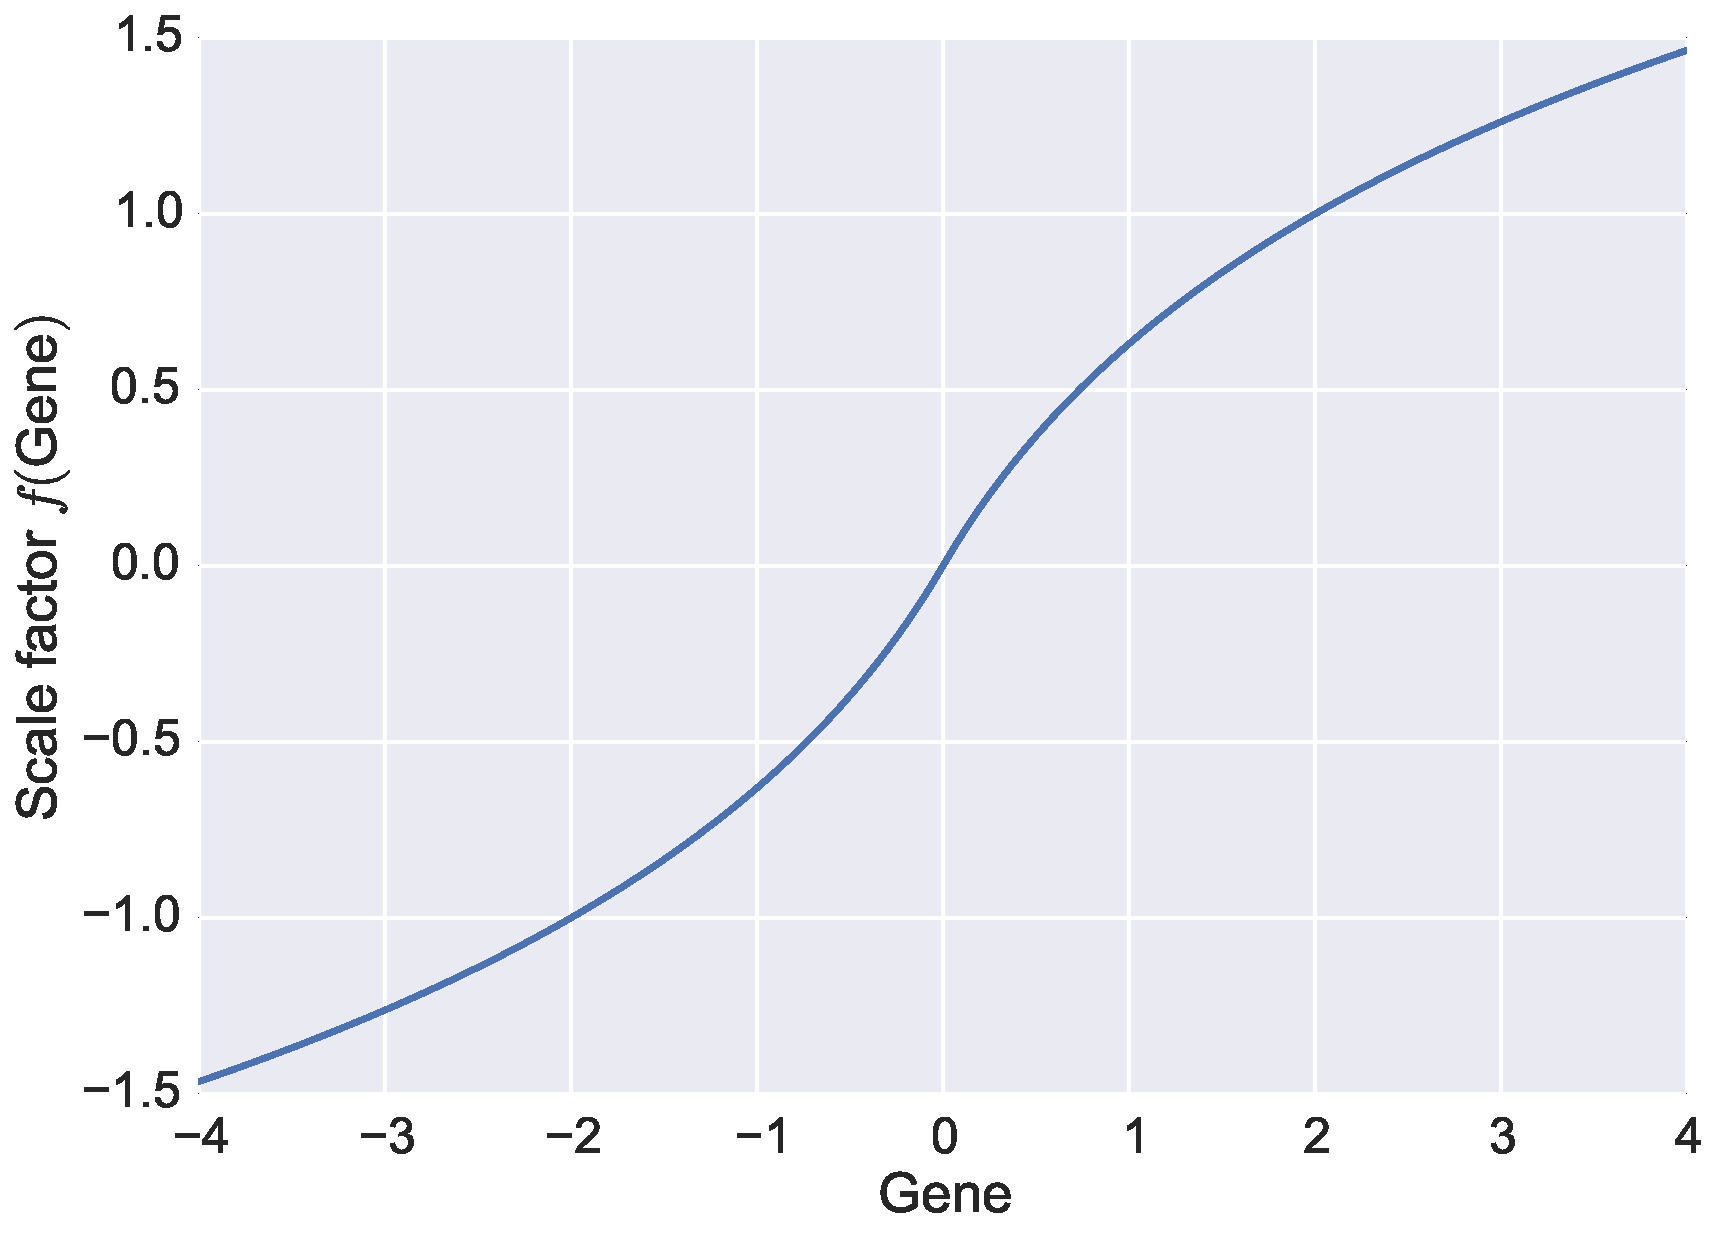
\includegraphics[width=.9\textwidth]{scale}
	\caption{Scale function $f$}
	\label{fig:scale}
\end{figure}

\section{Parameter Overview}
Here, the parameters of the model as defined in the file \verb+constants.py+ are explained:

\vspace{20pt}
\begin{tabularx}{\linewidth}{l | l | X}
Parameter & Type & Meaning \\ \midrule
population\_size & int & Number of animals per population. \\
generations & int & Number of generations per run. \\
L & int & Life time of each animal in time steps. \\
kd & float & Constant cost of plasticity. \\
ka & float & Cost of each adaptation. \\
tau & float & Coefficient of lifetime payoff exponential. \\
q & float & Controls expected number of offspring in variable scenario. \\
mu & float & Mutation rate of the genes. \\
environments & [[5$\times$float]] & Parameters of each environment in the order $R$, $P$, $A$, $B$, $O$. \\
environment\_names & [string] & Displayed name of each environment. \\
\modfont{km} & float & Cost of migration. \\
\modfont{limit} & [string] & Names of genes that should be limited to $[0,1]$. \\
populations & int & Number of identical populations per run. \\
plot\_every & int & Detailed output is plotted every N generations (0 = never). \\
verbose & bool & Triggers verbose output to command line.
\end{tabularx}
\vspace{20pt}

\noindent For more information, refer to the original paper, \cite{botero}. All parameter names are unchanged.
\section{Examplary Results}

\subsection{Final states}
Some final states for the standard parameters, but with different values of $R$ (the same for all environments):
\begin{description}
\item{$\mathbf{R=1}$:} \\
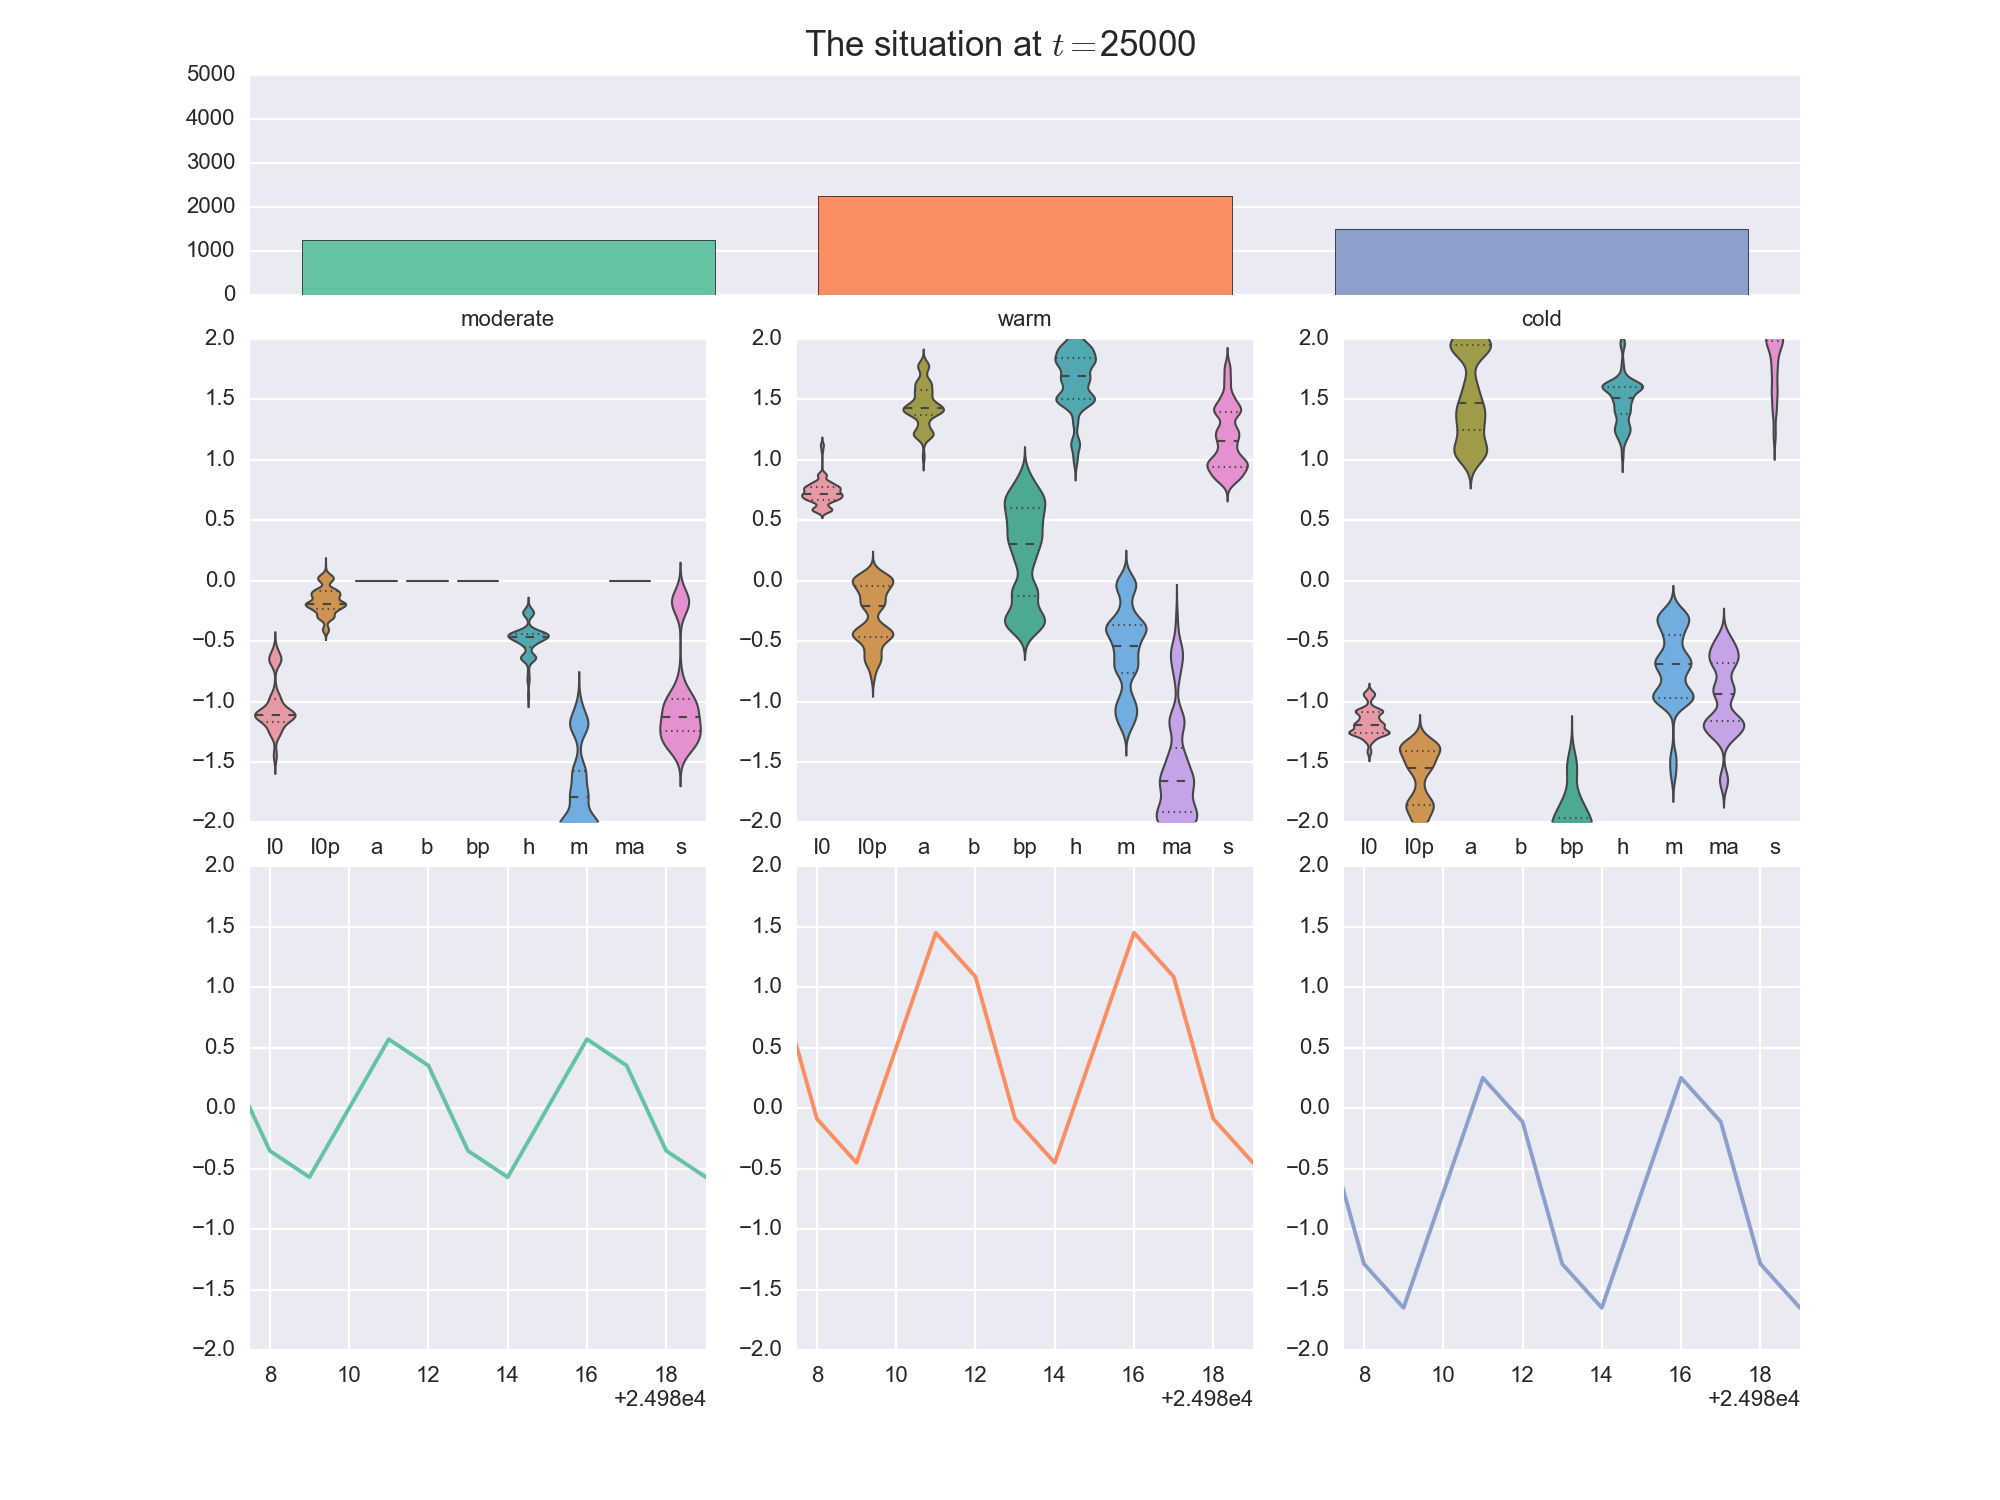
\includegraphics[width=\linewidth]{R1/end.png}
The animals in the moderate environment (which has low predictability) develop a conservative bet-hedging strategy, while the animals in the other, more extreme (but more predictable) environments develop reversible plasticity.

\item{$\mathbf{R=10}$:} \\
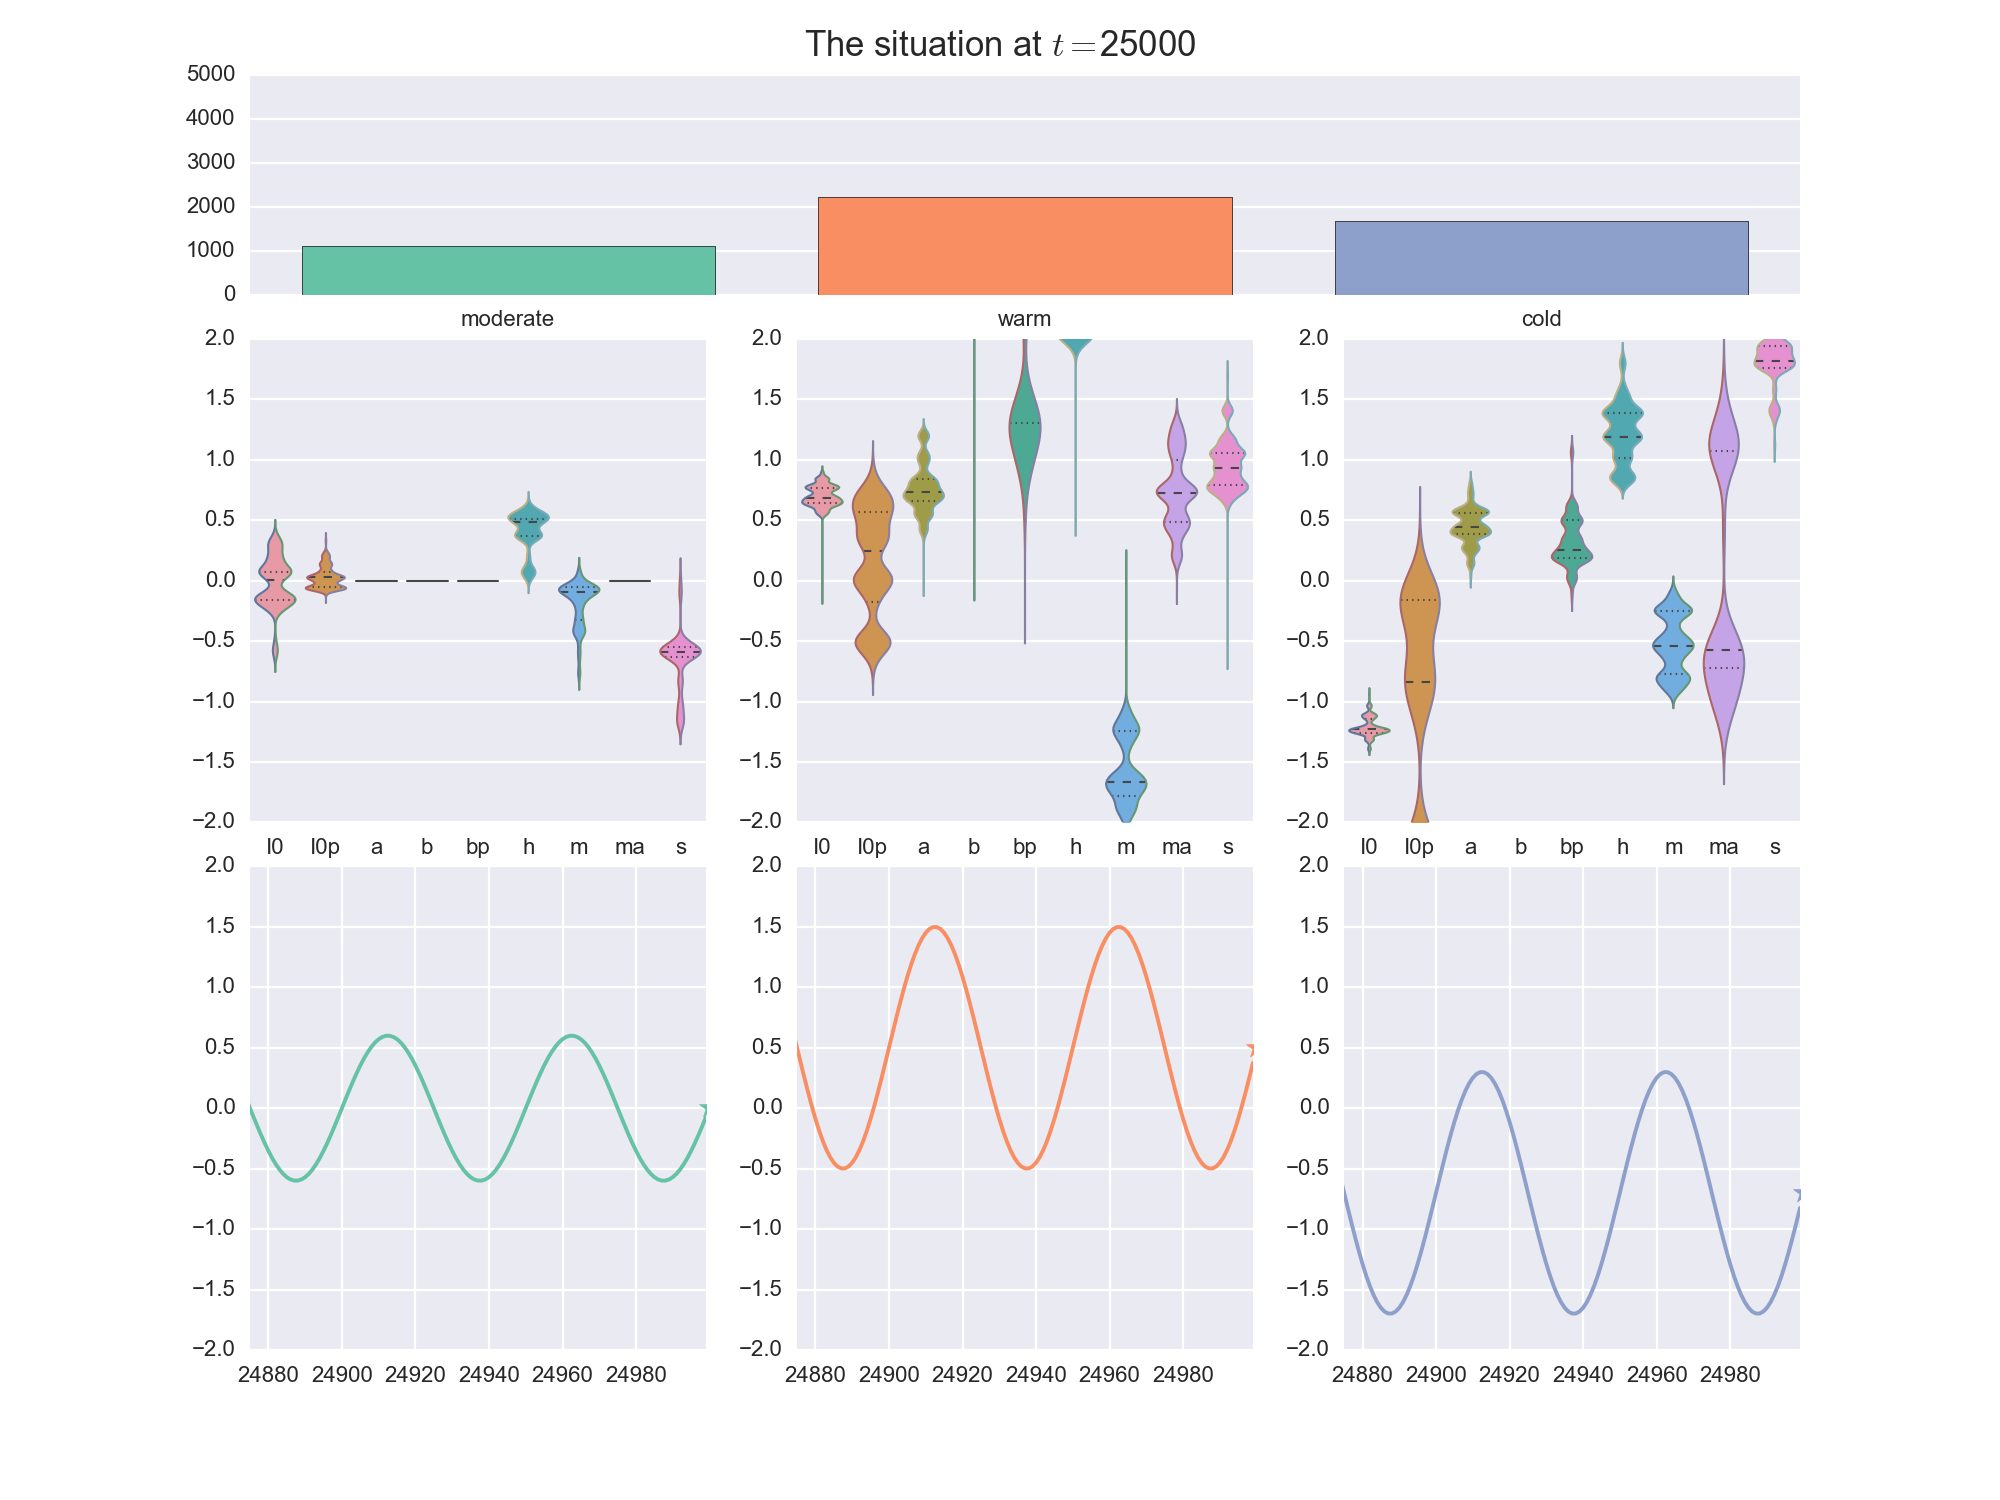
\includegraphics[width=\linewidth]{R10/end.png}
The moderate environment still shows conservative bet-hedging. The warm and cold environments show reversible plasticity of a lesser degree (smaller $a$).

\item{$\mathbf{R=100}$:} \\
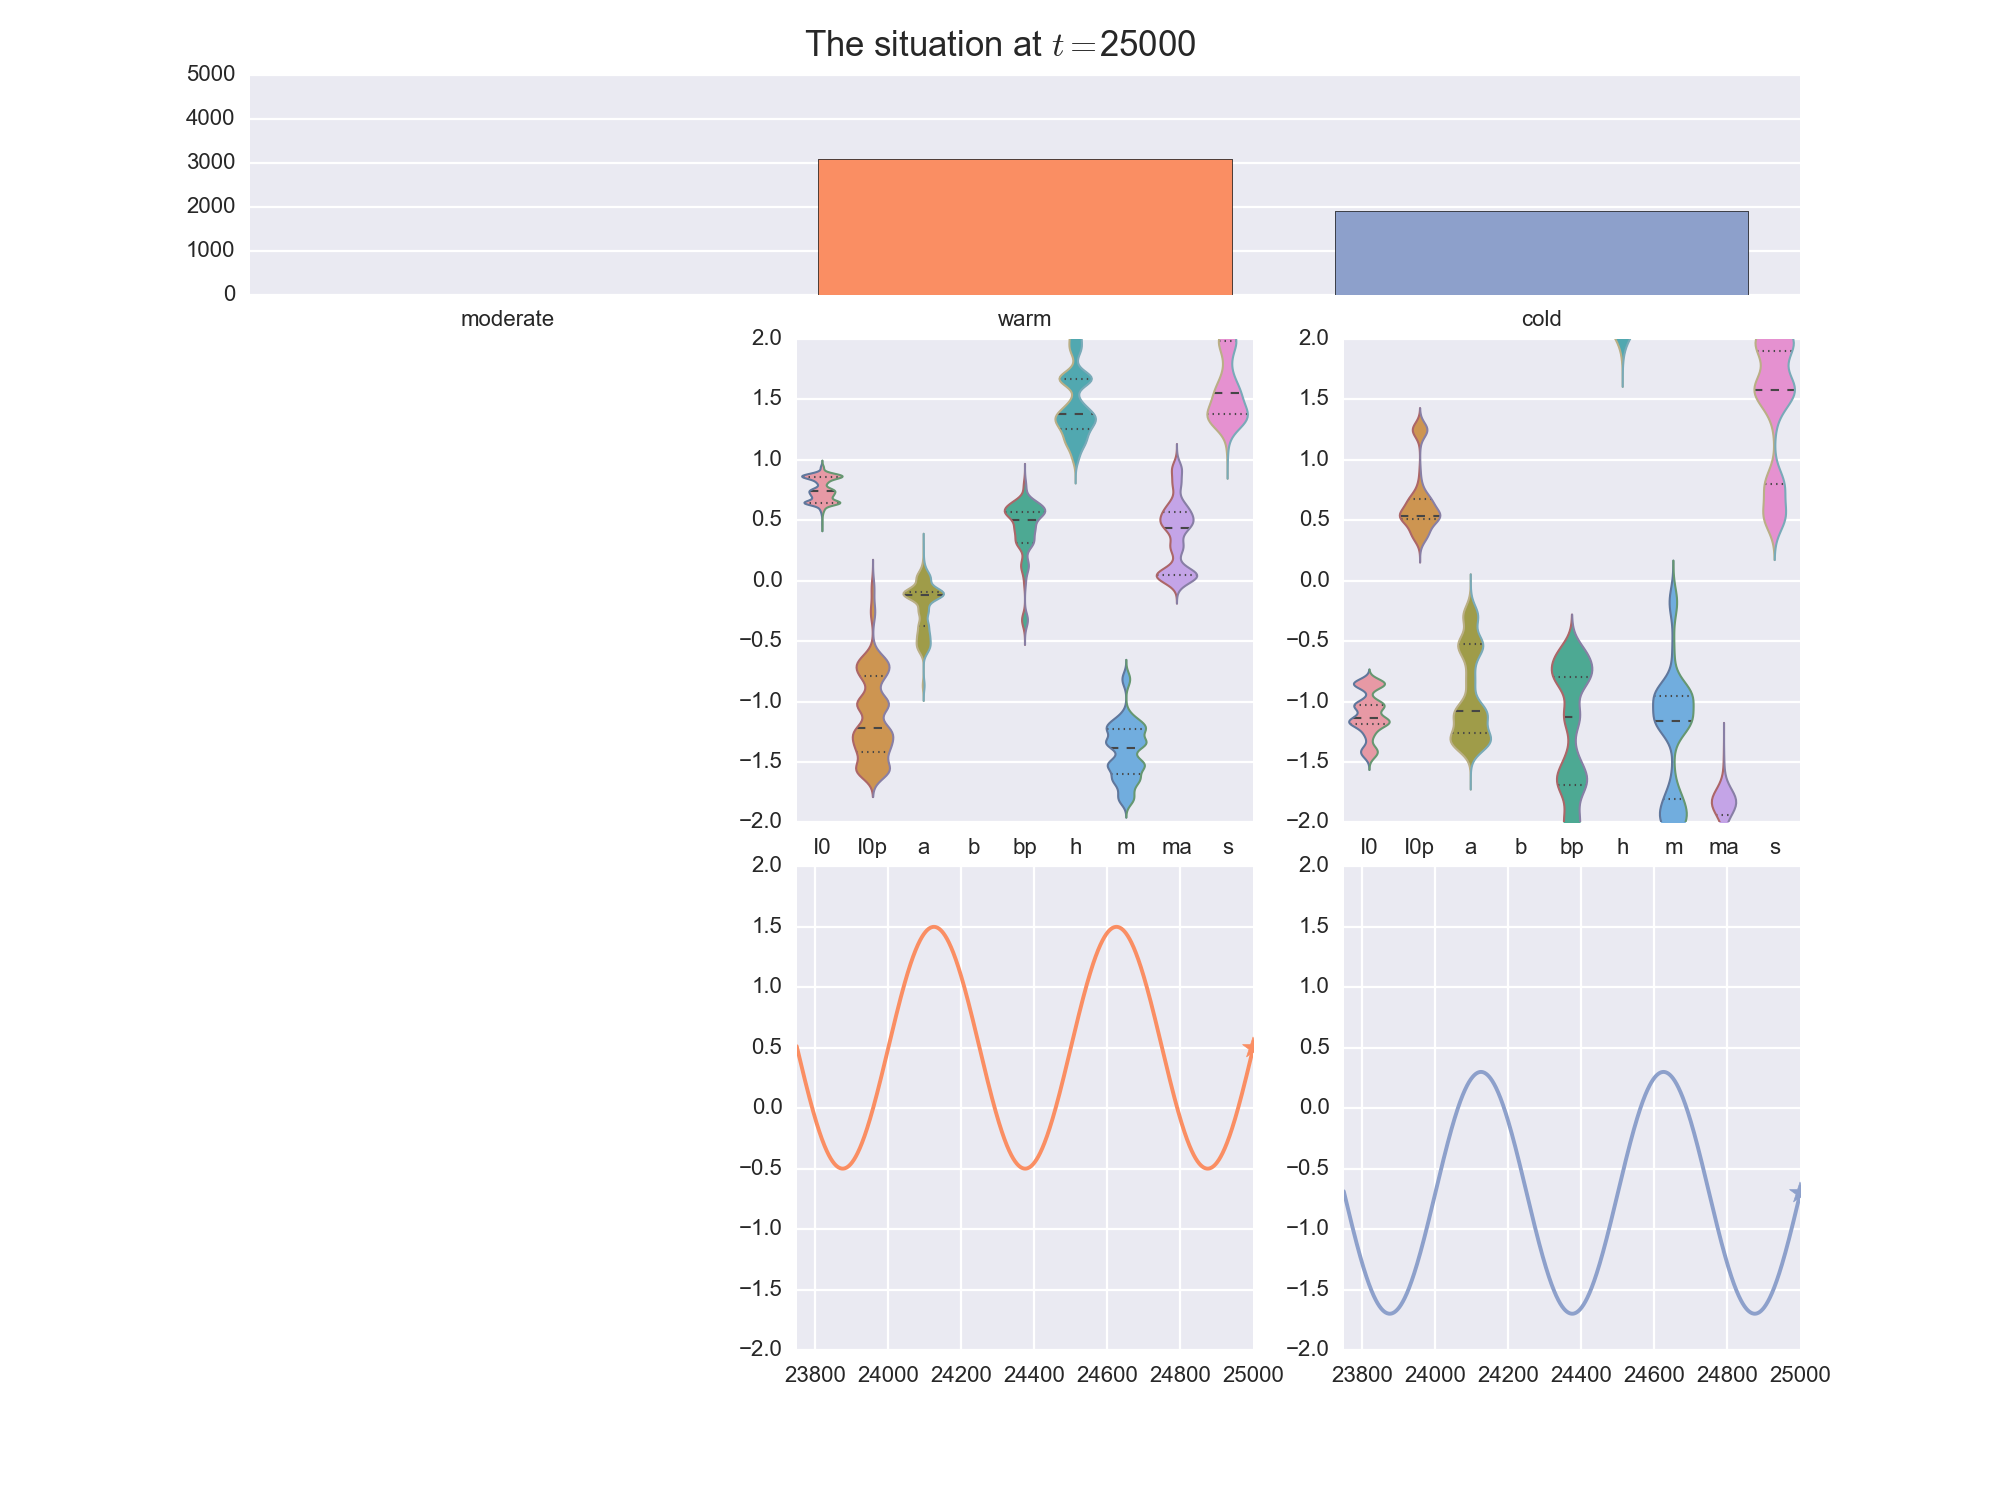
\includegraphics[width=\linewidth]{R100/end.png}
The animals in the moderate environment die out, the other environments show irreversible plasticity. The animals in the warm environment are more successful, since it is more predictable.

\item{$\mathbf{R=1000}$:} \\
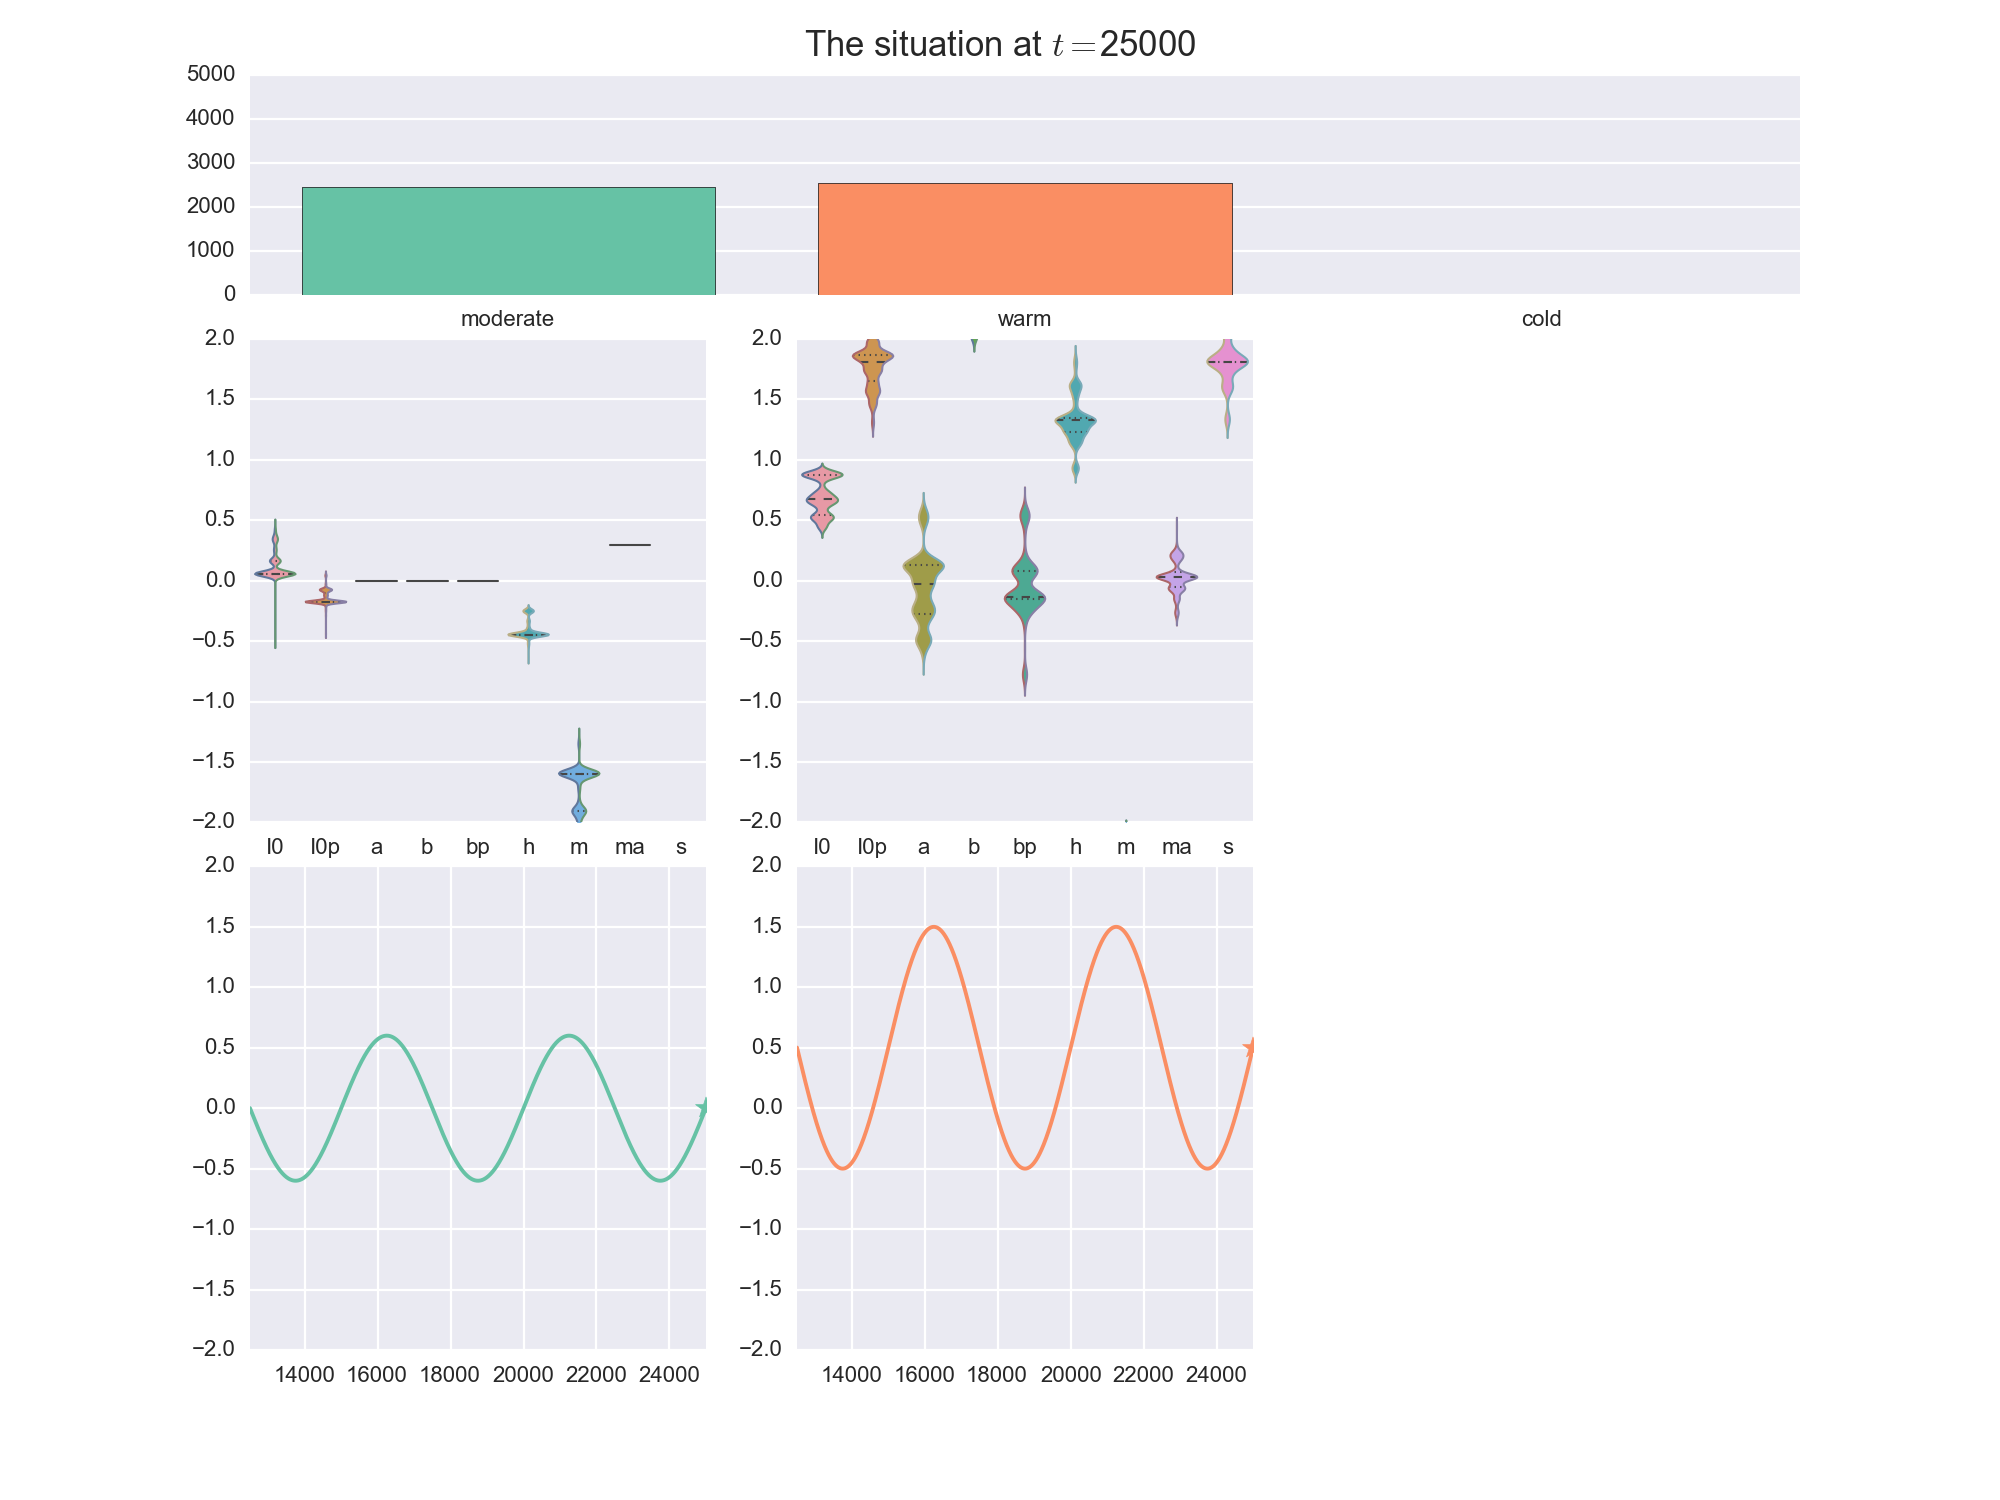
\includegraphics[width=\linewidth]{R1000/end.png}
The moderate environment shows adaptive tracking, while the animals in the warm environment develop a mixed strategy (adaptive tracking and irreversible plasticity). The animals in the cold environment die out. This is probably caused by the scale function $f$, which punishes adaptive tracking for extreme climates.
\end{description}

\subsection{Observed strategies}
The following figure shows the position of the standard environments in parameter space, and the strategies found in the final states during test runs for various combinations of $(P,R)$:

\centerline{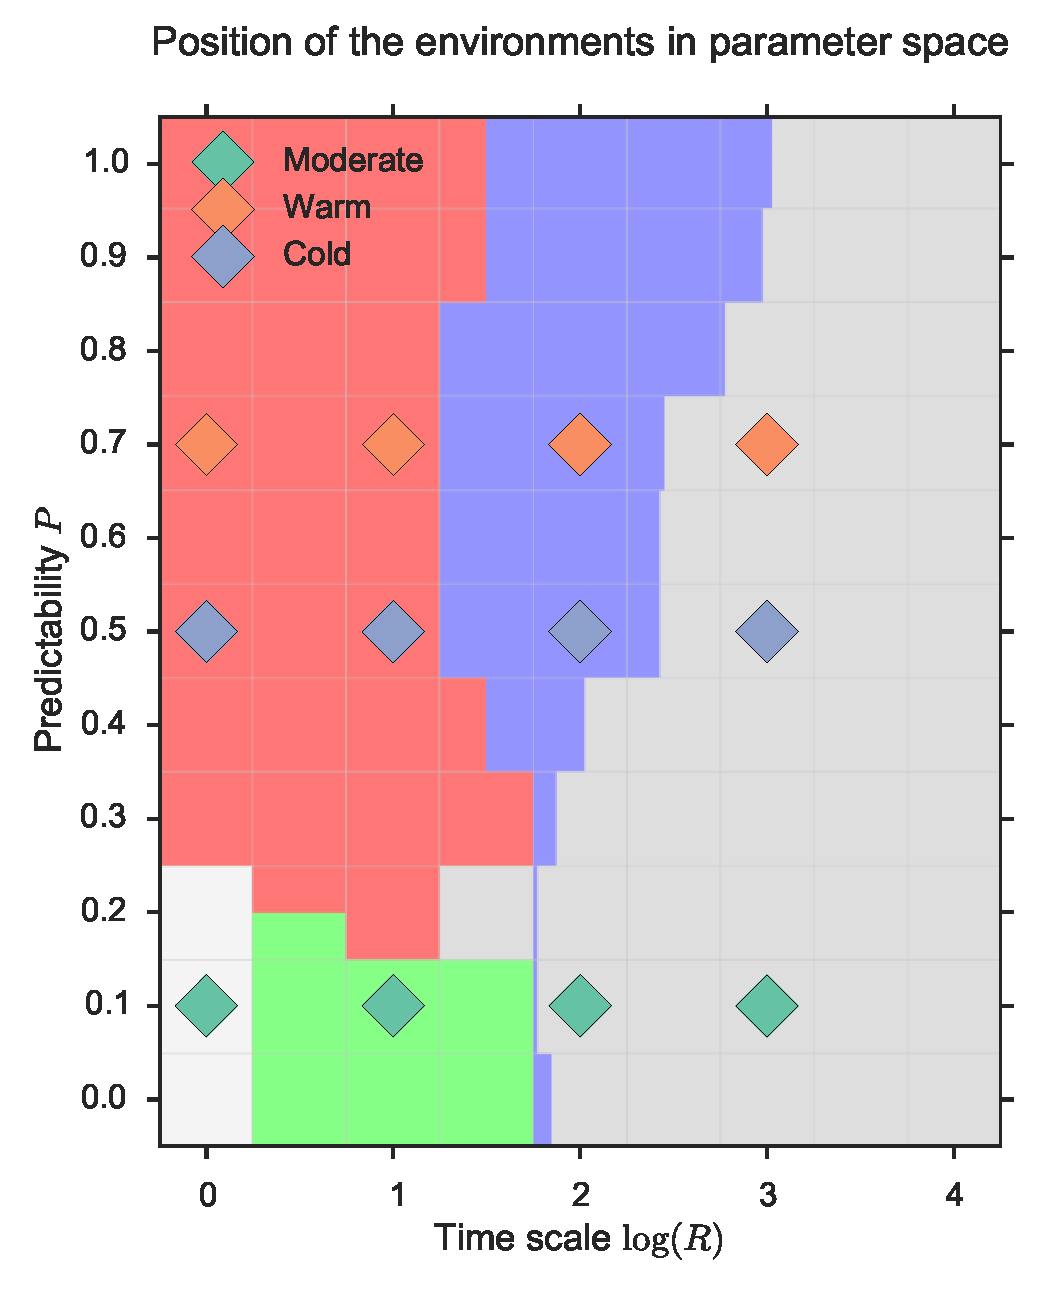
\includegraphics[width=.8\linewidth]{paraspace_axis}}

\noindent\textbf{Color-coding:}
\begin{description}
	\item[white:] conservative bet-hedging,
	\item[green:] diversifying bet-hedging,
	\item[red:] reversible plasticity,
	\item[blue:] irreversible plasticity,
	\item[grey:] adaptive tracking.
\end{description}

\subsection{Tipping points}
The following figure shows statistics on how many animals of a population (coming from environments with parameters $(P_i,~R), ~i\in\left\{1,2,3\right\}$) survived when put into environments with parameters $(P_i + \Delta P,~R')$ during a run with variable population size:
  
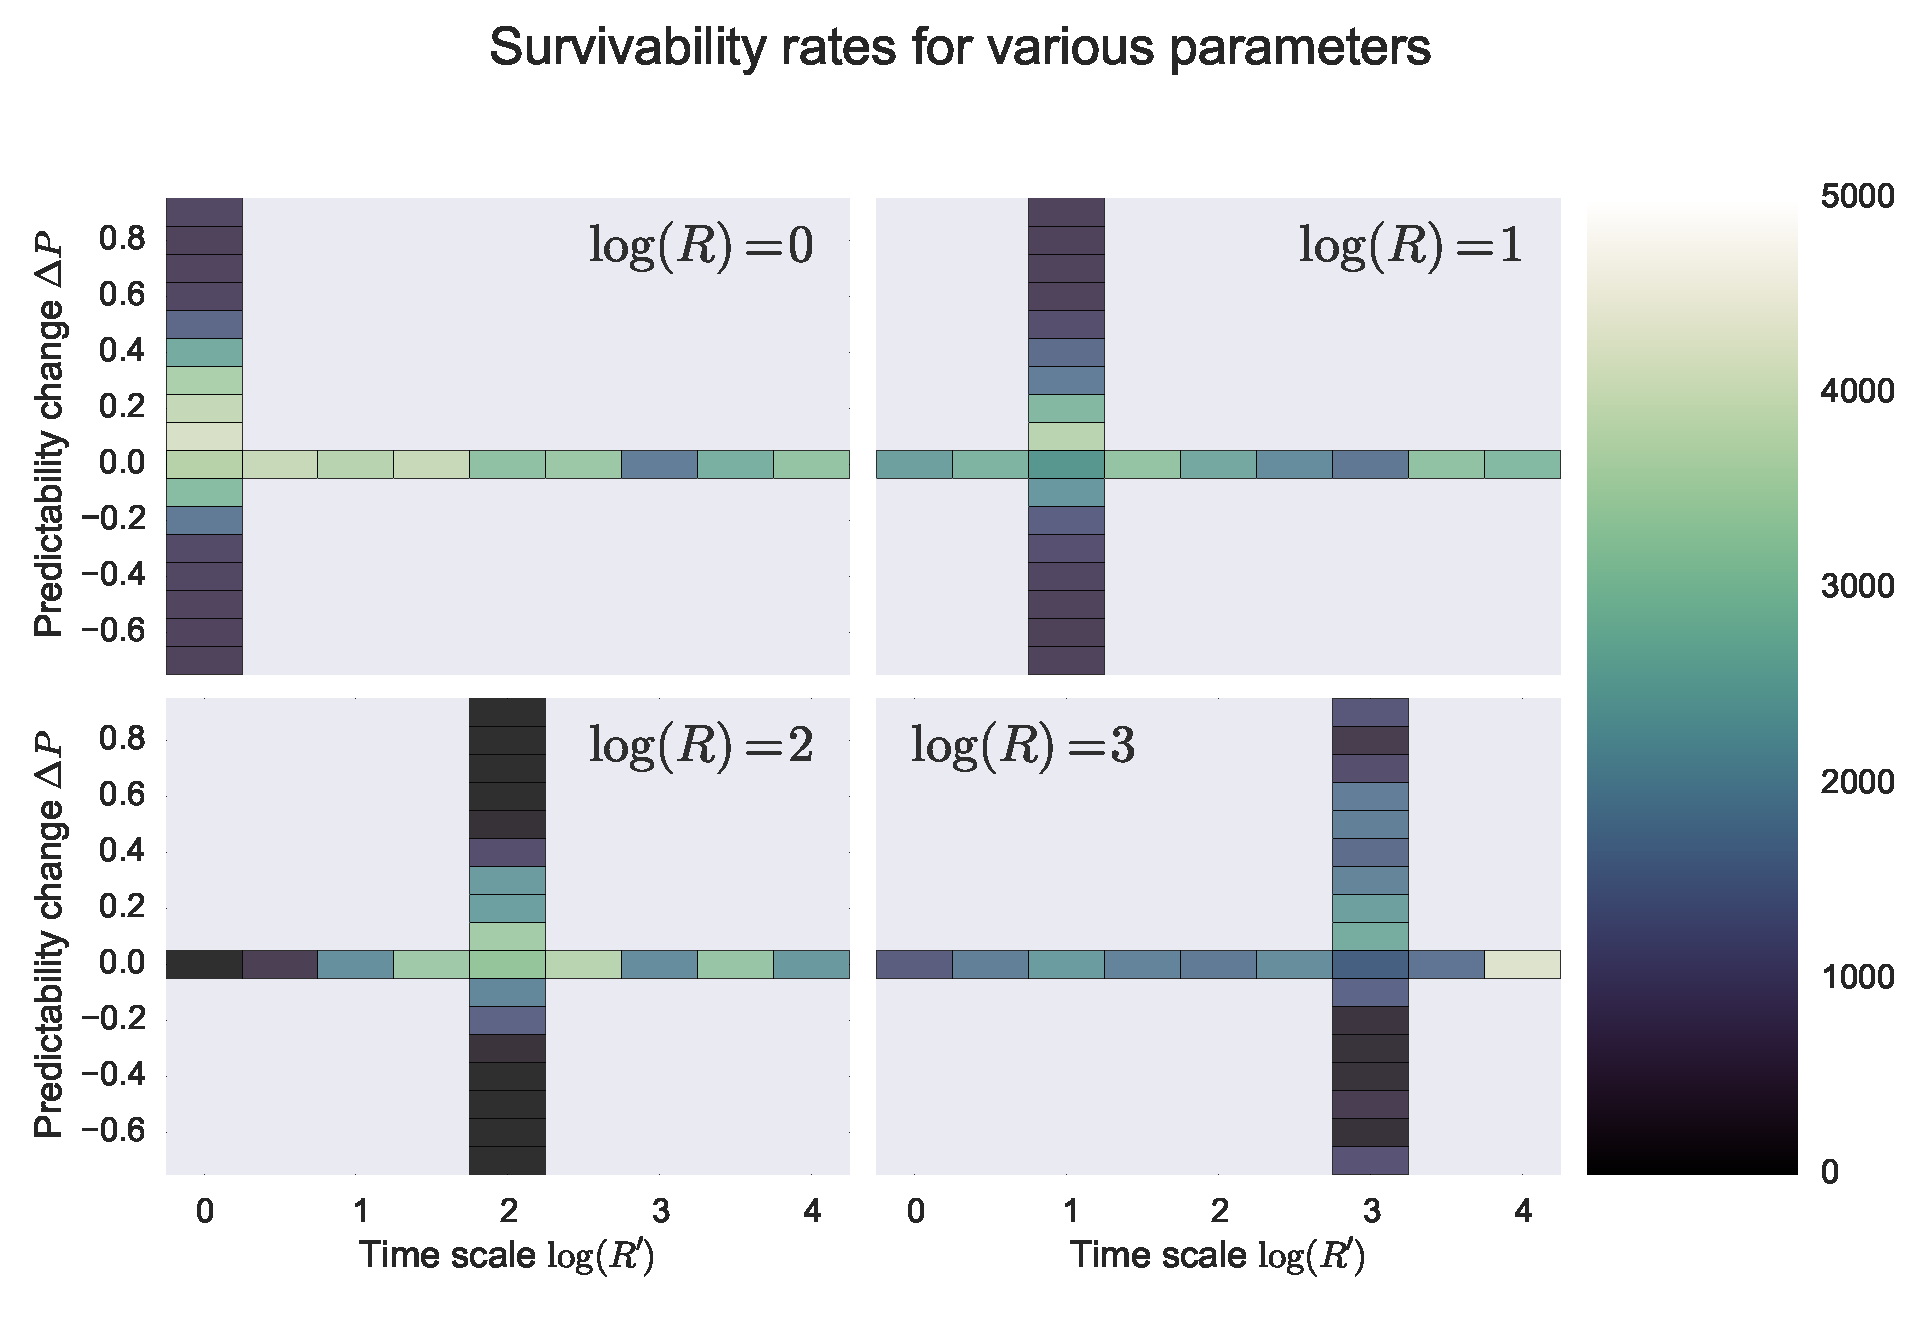
\includegraphics[width=\linewidth]{tipping}

\begin{thebibliography}{99}
  \bibitem{botero}
  Carlos A. Botero, Franz J. Weissing, Jonathan Wright, and Dustin R. Rubenstein:
  \newblock Evolutionary tipping points in the capacity to adapt to environmental change.
  \newblock {\em PNAS}, 112 (1): 184-189, 2015. \\
  \newblock \url{http://www.pnas.org/content/112/1/184}
\end{thebibliography}

\section*{License}
Copyright (c) 2015, Dion H\"afner.
All rights reserved.

Redistribution and use in source and binary forms, with or without modification, are permitted provided that the following conditions are met:

\begin{enumerate}
	\item Redistributions of source code must retain the above copyright notice, this list of conditions and the following disclaimer.
	
	\item Redistributions in binary form must reproduce the above copyright notice, this list of conditions and the following disclaimer in the documentation and/or other materials provided with the distribution.
\end{enumerate}

THIS SOFTWARE IS PROVIDED BY THE COPYRIGHT HOLDERS AND CONTRIBUTORS "AS IS" AND ANY EXPRESS OR IMPLIED WARRANTIES, INCLUDING, BUT NOT LIMITED TO, THE IMPLIED WARRANTIES OF MERCHANTABILITY AND FITNESS FOR A PARTICULAR PURPOSE ARE DISCLAIMED. IN NO EVENT SHALL THE COPYRIGHT HOLDER OR CONTRIBUTORS BE LIABLE FOR ANY DIRECT, INDIRECT, INCIDENTAL, SPECIAL, EXEMPLARY, OR CONSEQUENTIAL DAMAGES (INCLUDING, BUT NOT LIMITED TO, PROCUREMENT OF SUBSTITUTE GOODS OR SERVICES; LOSS OF USE, DATA, OR PROFITS; OR BUSINESS INTERRUPTION) HOWEVER CAUSED AND ON ANY THEORY OF LIABILITY, WHETHER IN CONTRACT, STRICT LIABILITY, OR TORT (INCLUDING NEGLIGENCE OR OTHERWISE) ARISING IN ANY WAY OUT OF THE USE OF THIS SOFTWARE, EVEN IF ADVISED OF THE POSSIBILITY OF SUCH DAMAGE.
\end{document}